% Pour vérifier qu'on écrit du LaTeX moderne
% \RequirePackage [orthodox] {nag}

\documentclass [twoside,openright,a4paper,11pt,french] {report}

    % Règles de typographie françaises
    \usepackage[french]{babel}

    % Jeu de caractères UTF-8
    \usepackage[utf8]{inputenc}
    \usepackage[T1]{fontenc}

    % Inclure la bibliographie dans la table des matières comme une section
    \usepackage [numbib] {tocbibind}	% numbib : section numérotée

    % Fonte élégante
    \usepackage {mathpazo}
    \usepackage [scaled] {helvet}
    \usepackage {courier}

    % pour certains symboles mathématiques peu fréquents, dont \square
    \usepackage {amssymb}

    % pour \EUR
    \usepackage {marvosym}

    % \usepackage {emptypage}

    % Utilisation de tableaux
    \usepackage {tabularx}

    % Utilisation d'url
    \usepackage {hyperref}
    \urlstyle {sf}

    % Utilisation d'images
    \usepackage{graphicx}
    \setkeys {Gin} {keepaspectratio}	% par défaut : conserver les proportions

    % Définition des marges
    \usepackage [margin=25mm, foot=15mm] {geometry}

    \parskip=2mm
    \parindent=0mm

    \pagestyle {plain}

\begin{document}

%%%%%%%%%%%%%%%%%%%%%%%%%%%%%%%%%%%%%%%%%%%%%%%%%%%%%%%%%%%%%%%%%%%%%%%%%%%%%%
% Page de garde
%%%%%%%%%%%%%%%%%%%%%%%%%%%%%%%%%%%%%%%%%%%%%%%%%%%%%%%%%%%%%%%%%%%%%%%%%%%%%%

\thispagestyle{empty}

\begin{center}
    % le ".1" est juste là pour montrer qu'on peut mettre des
    % dimensions non entières...
    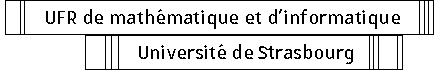
\includegraphics [width=8.1cm] {logo-ufr.pdf}       

    \vfill\vfill

    {
	\large
	\textsc {
	    Licence master 4 de Science, mention Informatique \\
	    parcours Sciences et Ingénierie des Réseaux, de l'Internet et des Systèmes
	}
    }

    \bigskip\bigskip

    {\large Mémoire de stage présenté par}

    \medskip

    % Identité de l'auteur
    {\large Jacques \textsc {Sélère}}

    % Contact mail ou téléphone   
    {\small jselere@unistra.fr}

    \vfill

    % Titre du stage : mettez un titre utile
    {
	\huge
	\textsc {
	    Comment faire un bon \\
	    ~ \\
	    mémoire de stage ?
	}
    }

    \vfill

    \today

    \vfill

    {\large Stage encadré par}

    \medskip

    % Identité de l'encadrant
    {\large Jean \textsc {Breille}}

    % Contact mail ou téléphone
    {\small +33 (0) 3.68.85.98.76}

    \bigskip

    {\large Au sein de}

    \medskip

    % Structure d'accueil
    {
	\large
	\textsc {Société de propulsion aéroportée des escargots}
    }

    \bigskip
    \bigskip

    % Logo de votre structure d'accueil
    
\includegraphics [height=2.5cm] {logo-entreprise.pdf}       

    % Supprimez le reste de cette page si vous vous servez de ce
    % fichier source comme modèle
    \vfill
    \begin {center}
	\tiny
	\copyright Pierre David,
	avec des contributions de 
	Cristel Pelsser, Stéphane Cateloin et Vincent Loechner

	Disponible sur \url {https://gitlab.com/pdagog/ens}.

        Ce texte est placé sous licence « Creative Commons Attribution
	-- Pas d’Utilisation Commerciale 4.0 International » \\
	Pour accéder à une copie de cette licence,
	merci de vous rendre à l'adresse suivante
	\url {https://creativecommons.org/licenses/by-nc/4.0/}

	
\includegraphics [scale=.5] {by-nc}
    \end {center}
    % Supprimez jusqu'ici


\end{center}

% Page blanche au dos de la page de garde
%\cleardoublepage

%%%%%%%%%%%%%%%%%%%%%%%%%%%%%%%%%%%%%%%%%%%%%%%%%%%%%%%%%%%%%%%%%%%%%%%%%%%%%%
% Table des matières
%%%%%%%%%%%%%%%%%%%%%%%%%%%%%%%%%%%%%%%%%%%%%%%%%%%%%%%%%%%%%%%%%%%%%%%%%%%%%%

{
    \parskip=0pt
    \tableofcontents
}

% Page blanche entre la table des matières et le texte
\cleardoublepage

%%%%%%%%%%%%%%%%%%%%%%%%%%%%%%%%%%%%%%%%%%%%%%%%%%%%%%%%%%%%%%%%%%%%%%%%%%%%%%
% Chapitre 1
%%%%%%%%%%%%%%%%%%%%%%%%%%%%%%%%%%%%%%%%%%%%%%%%%%%%%%%%%%%%%%%%%%%%%%%%%%%%%%

\chapter {Introduction}
    \label {chap:intro}

Le mémoire est un élément essentiel de votre stage : il a pour objet
d'exposer, le plus fidèlement possible, à la fois le périmètre du
stage (périmètres organisationnel et/ou technique) et votre contribution.

Votre mémoire sera lu par un «~rapporteur~», c'est-à-dire un
enseignant de l'équipe pédagogique (donc une personne ayant des
compétences dans votre discipline), dont la mission est d'évaluer votre
mémoire pour comprendre le contexte dans lequel vous avez évolué,
et votre contribution (réalisation technique, travail scientifique ou
autre) ainsi que son adéquation vis-à-vis de la formation.

Il est rappelé que le plagiat est sanctionné par la loi, par
l'université et par vos rapporteurs : si les courtes citations sont
autorisées, vous devez en donner la source.

Ce document a pour but de rappeler les éléments attendus par le
rapporteur pour évaluer votre travail. Il est de votre intérêt de
fournir tous ces éléments. Pour vous aider, des listes de points
à vérifier tant pour le mémoire que pour la soutenance sont
fournies en annexes de ce document.

Enfin, le source\footnote{Voir le répertoire \texttt{mem-stage/} sur
\url{https://gitlab.com/pdagog/ens}} de ce document est destiné à vous
servir de modèle si vous souhaitez rédiger votre mémoire avec \LaTeX.

%%%%%%%%%%%%%%%%%%%%%%%%%%%%%%%%%%%%%%%%%%%%%%%%%%%%%%%%%%%%%%%%%%%%%%%%%%%%%%
% Chapitre 2 : le plan
%%%%%%%%%%%%%%%%%%%%%%%%%%%%%%%%%%%%%%%%%%%%%%%%%%%%%%%%%%%%%%%%%%%%%%%%%%%%%%

\chapter {Le plan}
    \label {chap:plan}

Votre mémoire doit être bien structuré, c'est-à-dire présenter une
progression logique et apparente. Le plan est de votre responsabilité,
mais il doit comporter des chapitres relativement équilibrés (en taille)
et contenir les éléments décrits ci-après (un élément n'est pas
forcément un chapitre en soi). Les enchaînements entre les chapitres
et les sections doivent être compréhensibles.

N'omettez pas la table des matières, et numérotez vos chapitres et
vos sections (1, 1.1, 1.1.1, etc.), cela aide à se repérer. Et bien
évidemment, numérotez les pages, sinon ça ne sert à rien.

\section {L'organisme d'accueil}

L'exercice consiste à présenter une description de votre contexte
organisationnel : votre rapporteur ne connaît à priori pas
l'organisme d'accueil, donc vous devez le présenter à travers sa
branche d'activité, ses chiffres caractéristiques. De plus, vous
devez présenter votre place dans l'organisme : vous devez suivre une
description en «~entonnoir~» (voir figure~\ref {fig:entonnoir}),
c'est-à-dire partir de l'organisme dans son ensemble pour arriver
jusqu'à votre place en tant que stagiaire. Un organigramme peut aider
à comprendre votre place dans l'organisme ou le service concerné.

\begin {figure} [htbp]
    \begin {center}
	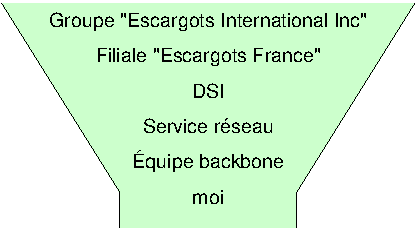
\includegraphics [width=.35\textwidth] {entonnoir.pdf}
    \end {center}
    \label {fig:entonnoir}
    \caption {Description de l'organisme : du plus large jusqu'à vous.}
\end {figure}

La figure~\ref {fig:entonnoir} présente la démarche : évoquer le
groupe au plus haut niveau (ses activités, son chiffre d'affaires, sa
présence dans le monde, le nombre d'employés, etc.), puis présenter
la filiale française et ainsi de suite jusqu'à arriver à l'équipe
dans laquelle vous vous situez (en précisant ses missions, le nombre
de personnes, etc.) et votre place dans cette équipe.

Évitez de recopier un site Web : cela se voit et ça énerve souvent
le rapporteur. Rédigez un texte avec vos propres mots : même s'il y a
des maladresses, cela passera beaucoup mieux.

Notez que la présentation de la structure d'accueil est obligatoire,
même si vous savez que cette structure est bien connue de votre
rapporteur (par exemple pour un stage réalisé dans le laboratoire
ICube). L'exercice imposé est de présenter cette structure, et tous
les stagiaires sont évalués sur ce critère, sans exception.

\section {La ou les missions}
    \label {sec:mission}

En tant que stagiaire, vous avez une ou plusieurs missions définies
correspondant à la durée de votre stage. Le rapporteur ne connaît
vraisemblablement pas ces missions. Décrivez-les, de préférence assez
tôt dans le mémoire, en les mettant en perspective par rapport aux
besoins de l'organisme. De plus, donnez les contraintes particulières
(financières, technique ou autres) ainsi que les objectifs à atteindre,
qui permettront d'évaluer ou non la réussite du projet.

\section {Le contexte}

Le contexte technique ou organisationnel doit être présenté.
Rappelez-vous que votre rapporteur a une bonne maîtrise des concepts
techniques, mais qu'il n'a pas connaissance des contraintes particulières
liées à votre organisme d'accueil ou à son métier.

N'abusez pas du contexte : vous devez présenter le minimum pour permettre
au rapporteur de comprendre les contraintes spécifiques de votre stage
et votre contribution. Pas plus.

Enfin, évitez le \frquote{\emph{bullshit}} : les documents de
présentation des organismes abusent souvent de phrases toutes faites qui
ne veulent rien dire comme \frquote{l'entreprise X place ses clients au
cœur de ses préoccupations} ou encore \frquote{le laboratoire Y est un
laboratoire d'excellence caractérisé par le haut niveau scientifique
de ses équipes}. On attend de vous que vous restiez factuel.


\section {Votre contribution}

C'est la principale partie de votre mémoire : vous devez présenter votre
contribution (réalisation logicielle, système informatique, état de
l'art, méthode, algorithme, évaluation, etc.) de façon synthétique,
sans sombrer dans les détails techniques mais en n'éludant pas les
points concrets qui permettent au rapporteur d'avoir la vision la plus
exacte possible de ce que vous avez mis en œuvre. Ne passez pas
les difficultés auxquelles vous avez été confronté sous silence.

Soyez précis et factuel : technologies, algorithmes ou méthodes
employés, éléments quantitatifs permettant d'apprécier l'envergure
du projet, comparatifs réalisés, etc. Si vous avez travaillé en
coopération avec d'autres personnes (votre maître de stage, d'autres
personnes ou stagiaires), indiquez avec précision votre rôle et vos
réalisations.

La méthodologie avec laquelle vous procédez est l'un des principaux
critères d'évaluation de votre travail : les problèmes doivent
être analysés, les choix effectués (ou auxquels vous avez pris part)
doivent être explicités et justifiés.

Il arrive souvent que, comme stagiaire, les choix vous soient imposés :
vous vous insérez dans un contexte qui existait avant votre arrivée,
certains choix sont faits en amont ou implicitement. Vous devez
les expliciter, et montrer que vous en maîtrisez les tenants et les
aboutissants : en d'autres termes, vous devez justifier certains choix,
même si ce ne sont pas les vôtres, pour montrer votre compréhension
des enjeux.

\section {Votre bilan}

Le stage complète votre formation : vous devez prendre du recul pour
mettre en rapport votre stage avec les compétences acquises pendant votre
formation, et présenter les compétences complémentaires (techniques,
personnelles, comportementales, etc.) que vous avez acquises durant
le stage.

Le bilan doit montrer votre recul par rapport au stage : vous avez le
droit (voire le devoir) de jeter un regard personnel et critique sur
votre comportement, sur votre démarche, sur votre réalisation ou même
sur le contexte, les choix effectués ou l'organisme d'accueil.


%%%%%%%%%%%%%%%%%%%%%%%%%%%%%%%%%%%%%%%%%%%%%%%%%%%%%%%%%%%%%%%%%%%%%%%%%%%%%%
% Chapitre 3
%%%%%%%%%%%%%%%%%%%%%%%%%%%%%%%%%%%%%%%%%%%%%%%%%%%%%%%%%%%%%%%%%%%%%%%%%%%%%%

\chapter {La forme}
    \label {chap:contexte}

Un bon mémoire allie un fond de qualité et une forme parfaite. Quelques
règles de bon sens s'appliquent.

\section {Typographie}

La rédaction de textes obéit à des règles précises en
Français : cela s'appelle la «~typographie~» \cite{andre1990} et il
est intéressant de s'en imprégner pour donner à votre document un
aspect de qualité et éviter des erreurs grossières.

\section {L'orthographe et la grammaire}

L'orthographe et la grammaire sont des prérequis indispensables pour
la rédaction du mémoire. Si vous n'êtes pas sûr de vous, faites-vous
relire par un tiers. C'est dommage de perdre des points sur ce critère.

\section {Le style}

Même si votre mémoire de stage n'a pas comme objectif de décrocher
le prix Goncourt, vous devez faire attention au style :

\begin {itemize}
    \item faites des phrases construites, avec des verbes. Exemple vécu,
	à éviter : «~Il y a des problèmes. Par exemple le
	format~» (il n'y pas de verbe)~;

    \item ne parlez pas au lecteur. Exemple vécu, à éviter : «~je vais
	vous présenter~»~;

    \item employez une forme active : plutôt qu'écrire «~xyz a été
	réalisé~», utilisez «~j'ai réalisé xyz~»~;

    \item soyez précis : écrivez «~j'ai réalisé xyz~» plutôt que «~on a
	réalisé xyz~». N'oubliez pas que le rapporteur doit évaluer
	\textbf{votre} travail (et pas celui de votre maître de stage ou
	de vos collègues)~;

    \item évitez les mots inutiles («~la société xyz existe
	\emph{maintenant} depuis 1789~») ou, pire encore, les phrases
	inutiles («~au cours de ce stage, j'ai pu travailler avec
	plusieurs personnes dans quelques environnements divers et
	variés~»)~;

    \item dans la même lignée, n'abusez pas du pouvoir~: «~j'ai pu
	faire...~» est une tournure inutilement compliquée qui est
	remplaçable par «~j'ai fait...~». C'est la même chose pour le
	verbe «~permettre~», le plus souvent inutile~: «~le logiciel
	permet de faire...~» est remplaçable par la forme plus directe
	«~le logiciel fait...~».

    \item évitez le futur : tout ce qui est fait au moment de l'écriture
	du mémoire doit être rédigé au passé ou au
	présent. Réservez le futur pour ce qui n'est pas encore
	réalisé ou pour les perspectives.

\end {itemize}


\section {Numérotez}

Numérotez tout ce qui peut l'être : pages, chapitres, sections, figures,
tables, bibliographie. Laissez à votre logiciel le soin de numéroter
automatiquement, il le fera mieux que vous «~manuellement~». Utilisez
des références si vous devez mettre en relation plusieurs éléments
de votre discours (exemple fictif : voir la figure~\ref {fig:entonnoir}
page~\pageref {fig:entonnoir}, ou encore le chapitre~\ref {chap:plan}
et plus spécifiquement la section~\ref {sec:mission}, page~\pageref
{sec:mission}).


\section {Les illustrations}

Un petit dessin valant mieux qu'un grand discours, les schémas de
principe sont très appréciés par le rapporteur qui ne connaît
pas votre environnement. Quelques règles cependant sont à respecter :

\begin {itemize}
    \item numérotez et légendez vos figures (voir figure~\ref
	{fig:entonnoir}, page~\pageref {fig:entonnoir}, par exemple) ;
    \item référencez vos figures : une figure non référencée dans le
	texte ne sert à rien ;
    \item expliquez vos figures dans le texte : si une figure ne nécessite
	pas d'explications, cela signifie qu'elle est sans doute trop
	simple et n'a donc pas besoin de figurer dans votre mémoire ;
    \item la bonne taille pour les figures est celle où les caractères
	sont à peu près de la même taille que le reste du texte~;
    \item citez la provenance de vos figures, si elles ne sont pas de
	vous : il est parfaitement admis d'utiliser des figures
	réalisées par d'autres, si vous citez la provenance ;
    \item les logos de logiciels ou de produits sont à bannir : ils
	n'apportent rien à la compréhension de votre mémoire et ne font
	que prendre de la place inutile que vous pourriez utiliser pour
	mieux présenter votre contribution ;
    \item privilégiez (sauf peut-être pour les photos) un format
	«~vectoriel~» à un format «~bitmap~» : le bitmap prend
	de la place, peut être lent à s'afficher ou à s'imprimer,
	et ne permet pas de zoomer facilement ;
    \item vérifiez que vos figures sont lisibles lorsque vous imprimez
	votre mémoire, y compris lorsque vous imprimez sur une
	imprimante noir et blanc.
\end {itemize}

Les copies d'écran n'apportent généralement pas grand-chose : elles
contiennent trop d'informations inutiles et sont peu lisibles. De plus,
le message véhiculé est souvent très succinct, voire trop léger. Un
fichier de configuration, une commande ou son résultat doivent être
présentés, si c'est vraiment nécessaire, comme du texte et non comme
une copie d'écran.

\section {Le niveau de détail}

Trouver le bon niveau de détail est souvent facilité par les contraintes
qui vous sont imposées quant au nombre de pages.

Cependant, même si vous avez la place, évitez les recopies de code ou de
commandes. Si vous voulez vraiment en faire, commentez-les dans le texte
et évitez de faire des erreurs dans les recopies ! Ne les modifiez pas
dans le texte (sauf pour supprimer une sortie trop longue par exemple,
dans ce cas remplacez la partie supprimée par «~[...]~»). Évitez
les codes trop longs~: utilisez des annexes si nécessaire.


\section {La bibliographie}

La bibliographie constitue une partie importante de votre mémoire.
Elle constitue un critère de qualité du travail (avez-vous trouvé les
bonnes sources ? les documents sur lesquels vous vous appuyez sont-ils
sérieux ?). Vous devez indiquer les documents :

\begin {itemize}
    \item de référence que vous avez consultés dans votre recherche,
	pour vous familiariser avec votre sujet ou pour apprendre
	des techniques particulières ;
    \item que vous avez consultés pour effectuer vos choix ou mettre
	en œuvre un dispositif logiciel ou autre ;
    \item qui permettent au lecteur d'en savoir plus sur tel ou tel
	point de votre mémoire que vous ne pouvez davantage développer.
\end {itemize}

La bibliographie~\cite {savoirs2010} vient en annexe, elle doit donner
tous les renseignements nécessaires pour permettre au lecteur de
retrouver les documents concernés : auteur, titre du document ou de
l'ouvrage, éditeur, année de publication, URL si nécessaire, date de
consultation pour un site Web, etc.

Chaque document dans la bibliographie comporte une référence (un
numéro, une abréviation ou autre), que vous devez citer dans le texte :
un document non cité ne devrait pas apparaître dans la bibliographie.

%%%%%%%%%%%%%%%%%%%%%%%%%%%%%%%%%%%%%%%%%%%%%%%%%%%%%%%%%%%%%%%%%%%%%%%%%%%%%%
% Conclusion
%%%%%%%%%%%%%%%%%%%%%%%%%%%%%%%%%%%%%%%%%%%%%%%%%%%%%%%%%%%%%%%%%%%%%%%%%%%%%%

\chapter {Conclusion}
    \label {chap:conc}

Il est maintenant temps de rédiger votre mémoire, en vous aidant des
listes de points à vérifier dans les annexes \ref{checklist-mem} et
\ref{checklist-sout}. Puissent ces quelques
conseils vous guider afin de vous aider à présenter le mieux possible
tout le travail que vous avez effectué durant votre stage !


%%%%%%%%%%%%%%%%%%%%%%%%%%%%%%%%%%%%%%%%%%%%%%%%%%%%%%%%%%%%%%%%%%%%%%%%%%%%%%
% Annexe : soutenance
%%%%%%%%%%%%%%%%%%%%%%%%%%%%%%%%%%%%%%%%%%%%%%%%%%%%%%%%%%%%%%%%%%%%%%%%%%%%%%

\appendix
\chapter {La soutenance}

Même si ce document concerne en priorité votre mémoire de stage,
il n'est pas inutile de rappeler quelques conseils de bon sens
pour que votre soutenance se déroule le mieux possible.

\begin {enumerate}
    \item Ne reproduisez pas le mémoire dans votre présentation : vous
	n'avez ni la place, ni le temps. Détachez-vous du mémoire et
	repartez de zéro pour construire un nouveau discours tenant
	compte de la contrainte de temps.

    \item Travaillez sur les idées et les messages que vous voulez
	faire passer. Comptez une idée par diapo. Explicitez les idées,
	ne vous contentez pas de les suggérer.

    \item Ne surchargez pas le texte de votre présentation : ne faites
	pas de phrases, insistez plutôt sur quelques mots pour exposer
	vos idées.

    \item Si vous pouvez prendre des libertés avec la grammaire et
	ne pas mettre de phrases, vous n'êtes pas dispensé de respecter
	l'orthographe.

    \item Adoptez un fond sobre pour ne pas perturber votre message.
	Numérotez vos diapos.

    \item Faites des illustrations (schémas, figures, courbes) qui
	puissent être lues à plusieurs mètres de distance. N'hésitez
	pas à prendre des libertés avec votre style de présentation
	pour faire une figure en pleine page.

    \item Attention aux contrastes : votre présentation projetée dans
	une salle éclairée aura un contraste beaucoup moins bon que
	l'écran de votre portable. Évitez donc les couleurs pâles
	sur fond clair, ou les couleurs peu foncées sur fond sombre.

    \item Une de vos missions est de maintenir l'attention de votre
	auditoire. Pensez que les membres du jury ont déjà peut-être
	une dizaine de présentations à leur actif, ainsi qu'un bon
	repas... Vous devez les motiver pour vous écouter.

    \item Ne lisez surtout pas les diapos que vous présentez ou, pire
	encore, un texte que vous auriez préparé. Regardez l'assistance
	et non vos diapos.

    \item Respectez la durée de votre présentation, voir plus loin.

    \item Répétez. Répétez. Répétez. Répétez. Répétez. Répétez.
	Répétez. Répétez. Répétez. Répétez. Répétez. Répétez.

    \item Lors de la séance des questions, laissez les membres du jury
	aller jusqu'au bout de leurs questions, sans les
	interrompre. N'hésitez pas à prendre quelques secondes pour
	vous permettre de réfléchir à chaque question, voire de la
	reformuler pour vérifier que vous l'avez bien comprise.

\end {enumerate}

Si vous n'avez pas l'habitude de faire des présentations, vous trouverez
facilement un grand nombre de vidéos ou de tutoriels qui vous donneront
de bons conseils.

Les directives qui vous sont données pour la soutenance incluent la
durée de la présentation. Vous devez impérativement respecter cette
durée~: ne terminez pas trop en avance (vous n'avez donc rien à dire ?),
ne terminez pas trop en retard (vous ne savez pas synthétiser et tenir
compte d'une contrainte ?). Il arrive très souvent qu'il y ait un barème
pour la durée, comme l'illustre la figure~\ref{fig:duree-prez}~: par
exemple, si la consigne est une durée de 20 minutes, vous aurez 4 points
sur 4 si votre présentation dure entre 19' et 20'59", 3 points sur 4
si votre présentation dure entre 18' et 18'59" ou entre 21' et 21'29",
etc. Si vous dépassez trop, le président du jury coupera court à
votre présentation.

\begin {figure} [htbp]
    \label {fig:duree-prez}
    \begin {center}
	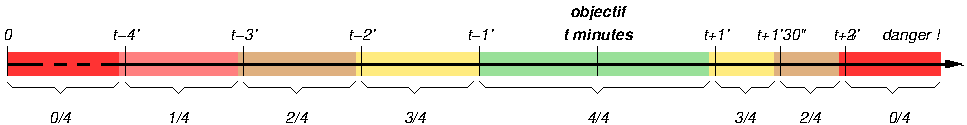
\includegraphics [width=\textwidth] {duree-prez.pdf}
    \end {center}
    \caption {Barème de la note (ici sur 4) en fonction de la durée
	de la présentation}
\end {figure}

%%%%%%%%%%%%%%%%%%%%%%%%%%%%%%%%%%%%%%%%%%%%%%%%%%%%%%%%%%%%%%%%%%%%%%%%%%%%%%
% Checklist mémoire
%%%%%%%%%%%%%%%%%%%%%%%%%%%%%%%%%%%%%%%%%%%%%%%%%%%%%%%%%%%%%%%%%%%%%%%%%%%%%%

\newenvironment{checklist}[1]{\vspace{-2.5ex}\section{#1}\vspace{-2ex}\begin{itemize}\vspace{-1ex}\small}{\end{itemize}}
\newcommand{\chkitem}[1]{\item [$\square$]#1}

\chapter {Checklist pour le mémoire}
    \label{checklist-mem}

Pour vous aider dans la rédaction du mémoire, voici une liste de
points à vérifier.  Une fois votre mémoire rédigé, vérifiez que
vous pouvez cocher \emph{toutes} les cases.

\begin{checklist}{Structuration du document}
\chkitem{Le titre du mémoire reflète ce que j'ai fait dans mon stage}
\chkitem{Le plan est clair et ne comporte pas d'allers-et-retours}
\chkitem{Les parties composant le mémoire sont de taille équilibrée}
\chkitem{Je respecte la limite de taille indiquée}
\chkitem{J'ai numéroté tous les chapitres, sections, sous-sections, etc. (1, 1.1, 1.1.1, etc.)}
\chkitem{J'ai numéroté toutes les pages (sauf la page de garde)}
\chkitem{Il y a une table des matières avec les numéros de page}
\chkitem{La lecture des annexes n'est pas nécessaire pour comprendre le travail que j'ai réalisé}
\chkitem{Tous les emprunts de texte/figure que j'ai faits sont dûment attribués à leurs auteurs respectifs}
\chkitem{Je mets l'accent sur la mise en œuvre des compétences attendues à mon niveau d'études, notamment l'esprit de synthèse, l'initiative et la maîtrise d'un problème complexe.}
\chkitem{Le maître de stage a validé mon mémoire}
\end{checklist}

\begin{checklist}{Présentation de l'entreprise}
\chkitem{J'ai présenté la structure d'accueil avec mes mots et j'ai évité de recopier un site web ou une plaquette commerciale}
\chkitem{La description de la structure d'accueil permet de comprendre son secteur d'activité, sa taille et son organisation}
\chkitem{Je donne des informations quantitatives lorsque cela permet de comprendre la dimension de la structure d'accueil et de son environnement}
\chkitem{Ma place dans la structure d'accueil est clairement explicitée et permet de comprendre les interactions avec mon environnement immédiat}
\end{checklist}

\begin{checklist}{Présentation des missions}
\chkitem{J'indique mes missions dès l'introduction, avant de les expliciter dans le reste du mémoire}
\chkitem{J'explicite la situation à mon arrivée, afin de bien faire comprendre la portée de ce que j'ai réalisé}
\chkitem{Je donne des informations quantitatives lorsque cela permet de comprendre la dimension du problème à résoudre}
\end{checklist}

\begin{checklist}{Présentation du travail effectué}
\chkitem{J'explicite les choix qui m'ont été imposés}
\chkitem{Je justifie tous les choix que j'ai effectués ou que j'ai contribué à effectuer}
\chkitem{En cas de travail partagé par plusieurs personnes, ma contribution personnelle est clairement explicitée}
\chkitem{Mon mémoire ne se limite pas à des descriptions techniques : je décris aussi les interactions avec les acteurs de mon stage : collègues, hiérarchie, clients, fournisseurs, prestataires...}
\chkitem{Plus que des étapes techniques, mon mémoire explicite la méthodologie que j'ai suivie}
\chkitem{Mes comparaisons sont plus claires avec un tableau de synthèse récapitulatif}
\chkitem{Je replace le travail effectué dans la stratégie de la structure d'accueil}
\end{checklist}

\begin{checklist}{Conclusions/réflexions}
\chkitem{Dans la conclusion, je donne des informations sur l'état du travail et son utilisation par la structure d'accueil}
\chkitem{Dans la conclusion, je donne des perspectives sur ce que pourrait être la suite du travail}
\chkitem{Je dresse le bilan des compétences acquises durant le stage, sans me limiter aux compétences techniques}
\end{checklist}

\begin{checklist}{Expression}
\chkitem{Je rédige le texte du mémoire et j'évite le style télégraphique ou les listes à puces sans phrases}
\chkitem{J'évite le style « parlé », chaque phrase comprend au moins un sujet, un verbe et un complément}
\chkitem{Je ne m'adresse pas directement au lecteur (« Je vais vous présenter mon travail »)}
\chkitem{Je ne passe pas à la ligne après chaque phrase et je respecte la règle « un paragraphe = une idée » }
\chkitem{Le texte de mon mémoire ne comprend aucun terme familier}
\chkitem{Je n'abuse pas des anglicismes : aucun des termes anglais restants n'a de traduction française bien acceptée}
\chkitem{J'utilise les verbes « permettre » et « pouvoir » à bon escient et avec parcimonie}
\chkitem{J'explicite les termes peu usuels}
\chkitem{J'emploie la première personne du singulier pour tout ce que j'ai fait moi-même}
\chkitem{J'emploie le présent ou le passé pour ce qui a été réalisé}
\chkitem{Je n'emploie le futur que pour ce qui n'est pas encore réalisé}
\chkitem{J'introduis les termes techniques ou les sigles peu courants en dehors de la structure d'accueil}
\chkitem{J'ajoute un lexique en fin de document pour récapituler les termes techniques ou les sigles lorsque j'en utilise beaucoup}
\end{checklist}

\begin{checklist}{Orthographe/grammaire}
\chkitem{J'ai passé le correcteur orthographique et grammatical... et j'ai corrigé les fautes}
\chkitem{J'ai fait relire le document par une personne maîtrisant l'orthographe et la grammaire}
\chkitem{Les URL figurant dans le mémoire (y compris dans la bibliographie) sont cliquables}
\end{checklist}

\begin{checklist}{Iconographie}
\chkitem{Chacune de mes figures est numérotée et légendée}
\chkitem{Les figures sont lisibles lorsqu'elles sont imprimées (sur papier) en noir et blanc}
\chkitem{Le texte dans les figures est de taille comparable au texte du mémoire}
\chkitem{Les copies d'écran ne comportant que du texte, les suites de commandes et les fichiers de configuration ne sont pas intégrés sous forme d'image, mais sous forme de texte}
\chkitem{Sauf cas particulier, toutes mes illustrations sont en format vectoriel}
\chkitem{Lorsque je ne peux pas faire autrement qu'intégrer une figure en « bitmap », je veille à ce qu'elle reste lisible}
\chkitem{Je ne place dans le mémoire que les figures indispensables à la compréhension}
\chkitem{J'indique les unités (appropriées) sur les graphiques}
\chkitem{J'ai cité chaque figure dans le corps du texte, avec une explication}
\chkitem{L'explication sur chaque figure indique bien ce que le lecteur est censé retenir de la figure}
\chkitem{Les concepts ardus ou les points spécifiques du stage sont illustrés avec des figures}
\end{checklist}

\begin{checklist}{Bibliographie}
\chkitem{J'ai ajouté une bibliographie pour que les personnes intéressées puissent approfondir certains sujets évoqués}
\chkitem{La bibliographie contient les références suffisantes pour accéder à tous les documents cités}
\chkitem{Tous les éléments référencés dans le texte sont indiqués dans la bibliographie}
\chkitem{Chaque élément de la bibliographie est cité au moins une fois dans le texte}
\end{checklist}

%%%%%%%%%%%%%%%%%%%%%%%%%%%%%%%%%%%%%%%%%%%%%%%%%%%%%%%%%%%%%%%%%%%%%%%%%%%%%%
% Checklist soutenance
%%%%%%%%%%%%%%%%%%%%%%%%%%%%%%%%%%%%%%%%%%%%%%%%%%%%%%%%%%%%%%%%%%%%%%%%%%%%%%

\chapter {Checklist pour la soutenance}
    \label{checklist-sout}

Comme pour le mémoire (voir annexe~\ref{checklist-mem},
page~\pageref{checklist-mem}), vous trouverez ci-après une liste de
points à vérifier pour réussir votre soutenance.

\begin{checklist}{Structuration}
\chkitem{Le titre de la présentation reflète ce que j'ai fait dans mon stage}
\chkitem{Le plan est clair et ne comporte pas d'allers-et-retours}
\chkitem{Les parties composant le diaporama sont de taille équilibrée}
\chkitem{La description de la structure d'accueil permet de comprendre le secteur d'activité, la taille, l'organisation, ainsi que l'environnement immédiat du stagiaire}
\chkitem{Ma place dans la structure d'accueil est clairement explicitée et permet de comprendre les interactions avec mon environnement immédiat}
\chkitem{Je donne des informations quantitatives lorsque cela permet de comprendre la dimension de la structure d'accueil et de son environnement}
\chkitem{Plus que des étapes techniques, j'explicite la méthodologie que j'ai suivie}
\chkitem{Le maître de stage a relu ma présentation}
\chkitem{J'ai répété ma présentation devant le maître de stage et j'ai intégré ses remarques}
\end{checklist}

\begin{checklist}{Présentation du contexte et des objectifs}
\chkitem{J'explicite la situation à mon arrivée, afin de bien faire comprendre la portée de ce que j'ai réalisé}
\chkitem{J'explicite les choix qui m'ont été imposés}
\chkitem{Je donne des informations quantitatives lorsque cela permet de comprendre la dimension du problème à résoudre}
\chkitem{J'introduis les termes techniques ou les sigles peu courants en dehors de la structure d'accueil}
\end{checklist}

\begin{checklist}{Présentation du travail réalisé}
\chkitem{Je justifie tous les choix que j'ai effectués ou que j'ai contribué à effectuer}
\chkitem{En cas de travail partagé par plusieurs personnes, ma contribution personnelle est clairement explicitée}
\chkitem{Je replace le travail effectué dans la stratégie de la structure d'accueil}
\end{checklist}

\begin{checklist}{Bilan, conclusion, réflexions}
\chkitem{Dans la conclusion, je donne des informations sur l'état du travail et son utilisation par la structure d'accueil}
\chkitem{Dans la conclusion, je donne des perspectives sur ce que pourrait être la suite du travail}
\chkitem{Je dresse le bilan des compétences acquises durant le stage, sans me limiter aux compétences techniques}
\end{checklist}

\begin{checklist}{Qualité des diapos}
\chkitem{Les diapos ne sont ni trop remplies, ni trop vides}
\chkitem{Le diaporama comporte du texte et des illustrations de manière équilibrée}
\chkitem{Le texte des diapos correspond à des points clefs, et non à des phrases complètes}
\chkitem{Tous les messages à destination de l'assistance sont explicités}
\chkitem{Tous les emprunts de texte/figure que j'ai faits sont dûment attribués à leurs auteurs respectifs}
\chkitem{J'ai passé le correcteur orthographique et grammatical... et j'ai corrigé les fautes}
\chkitem{J'ai fait relire le document par une personne maîtrisant l'orthographe et la grammaire}
\chkitem{Les diapos sont numérotées}
\chkitem{Les diapos sont sur un fond clair (ou mieux : blanc)}
\chkitem{Le diaporama comporte de nombreuses illustrations pour mieux faire comprendre les points délicats}
\chkitem{Mes illustrations véhiculent une idée ou un message à faire passer à l'auditoire, que j'explicite au moins oralement}
\chkitem{J'illustre avec des schémas les concepts ardus ou les points spécifiques de mon stage}
\chkitem{Dans les figures, les couleurs doivent être contrastées car la projection aplatit les couleurs}
\chkitem{Lors de la projection, le texte et les figures doivent pouvoir être lus au 5e rang de la salle}
\chkitem{Le texte dans les figures est de taille comparable au texte des diapos, et il reste lisible au 5e rang}
\chkitem{Les copies d'écran ne comportant que du texte, les suites de commandes et les fichiers de configuration ne sont pas intégrés sous forme d'image, mais sous forme de texte}
\chkitem{Lorsque je ne peux pas faire autrement qu'intégrer une figure en «~bitmap~», je veille à ce qu'elle reste lisible}
\chkitem{Sauf cas particulier, toutes mes illustrations sont en format vectoriel}
\chkitem{J'explicite les termes peu usuels}
\chkitem{Mes comparaisons sont plus claires avec un tableau de synthèse récapitulatif}
\end{checklist}

\begin{checklist}{Gestion du temps}
\chkitem{Je présente le plan}
\chkitem{Le temps est compté : plus long, c'est une pénalité}
\chkitem{Le temps est compté : plus court, c'est courir le risque de manquer de matière}
\chkitem{Je ne passe pas plus d'une minute ou deux par diapo}
\end{checklist}

\begin{checklist}{Élocution, discours, posture}
\chkitem{Ma tenue vestimentaire est adaptée au moment solennel que constitue la soutenance}
\chkitem{Je ne prends pas mes notes avec moi}
\chkitem{Je regarde l'assistance, et non mes notes ou mes diapos (sauf pour pointer un élément important)}
\chkitem{Je suis enthousiaste, je souris}
\chkitem{Je parle assez fort et distinctement}
\chkitem{J'impulse un rythme dynamique à mon discours}
\chkitem{Je fais attention à ne pas utiliser un langage familier}
\chkitem{Je fais attention à mes tics verbaux («~du coup~», «~en fait~»...)}
\chkitem{Je fais attention à ma posture : je ne me fige pas, mais je ne gigote pas}
\chkitem{J'emploie la première personne du singulier pour tout ce que j'ai fait moi-même}
\chkitem{J'emploie le présent ou le passé pour ce qui a été réalisé}
\chkitem{Je n'emploie le futur que pour ce qui n'est pas encore réalisé}
\chkitem{Je n'abuse pas des anglicismes : aucun des termes anglais que j'utilise n'a de traduction française bien acceptée}
\end{checklist}

\begin{checklist}{Réponses aux questions}
\chkitem{Une fois la présentation terminée, je laisse la projection active au cas où une question ferait référence à une diapo}
\chkitem{Je laisse les membres du jury terminer de poser leur question avant de commencer à répondre}
\chkitem{En cas de doute, je reformule la question pour être sûr de l'avoir bien comprise et ne pas risquer de répondre à côté}
\chkitem{Si je ne sais pas répondre à une question, je préfère dire que je ne sais pas plutôt que de répondre n'importe quoi}
\end{checklist}

%%%%%%%%%%%%%%%%%%%%%%%%%%%%%%%%%%%%%%%%%%%%%%%%%%%%%%%%%%%%%%%%%%%%%%%%%%%%%%
% Bibliographie
%%%%%%%%%%%%%%%%%%%%%%%%%%%%%%%%%%%%%%%%%%%%%%%%%%%%%%%%%%%%%%%%%%%%%%%%%%%%%%

\cleardoublepage
\bibliographystyle{plain}
\bibliography{memoire}

\end{document}
